\section{Reproducibility and validation}
\label{sec:reproducibility}
The run identifier is \texttt{circle-mature-online148-20261001/full}. Immutable bulk captures and recordings remain on workstation 148. The report source package retains the current configuration, native configuration identities, source and binary hashes, accuracy results, communication counters, timing summaries, and publication audits. Tables are generated directly from these saved JSON records; report generation does not rerun SLAM, fit trajectories or change acceptance thresholds.

Post-run inspection identifies workstation 148 as an Intel Core Ultra 9 285K host with 24 visible logical CPUs, approximately 62.25\,GiB OS-visible RAM, and an NVIDIA GeForce RTX 5080 (16,303\,MiB reported device memory). The retained inventory is labeled post-run; it is not a record of experiment-time clock rates or utilization.

The effective settings are summarized in Table~\ref{tab:settings}. Native calibrated frontend files and per-robot CBS YAML take precedence over inherited unused configuration fields. In particular, execution is persistent with a 0.1\,Hz requested update rate and 30 final settling iterations. The point-cloud renderer and terrain-relative retrieval policy define the reported backend.
\begin{table}[htbp]
\centering\small
\caption{Effective configuration of the reported online run.}
\label{tab:settings}
\begin{tabular}{lp{0.68\linewidth}}
\toprule
Component & Setting \\
\midrule
Odometry & Persistent native EllipseLIO; calibrated IMU frame \\
Circle footprint & Radius 40\,m; 1\,m occupied-cell grid; 99\% coverage \\
Placement priorities & Coverage, circle count, then 30\% overlap target \\
Placement solve limit & 10\,s per update; validated greedy fallback \\
Normal geometry publication & Age $\geq$30\,s; growth $\leq$5\% over $\geq$30\,s; terrain/feature gates \\
Forced publication & 120\,s deadline at next observation, or end of stream \\
BEV retrieval & Point density, 0.5\,m pixels; five terrain-relative bands \\
Point-GICP verification & 0.4\,m evidence voxels; 1.5\,m correspondence radius \\
PCM & Probability 0.99; minimum clique size one \\
Registration factors & Native GPU VGICP; 0.5\,m preprocessing; 12,000 points/endpoint \\
Factor voxel levels & Two adaptive levels; recorded maps at 1 and 2\,m \\
Persistent CBS & 0.1\,Hz requested; random outgoing pose/anchor exchange \\
Final settling & Common-reference barrier, then 30 iterations \\
Evaluation & evo 1.36.5; 50\,ms association; shared rigid alignment; no scale \\
\bottomrule
\end{tabular}
\end{table}


An independent audit reconstructs every published payload from its seal-time observation prefix, checking member IDs, coordinates, creation anchors, hashes and descriptor/evidence agreement. Graph-prefix checks establish causal availability and both-endpoint receipt before loop admission. All final admitted registration factors pass support checks; published loop transforms satisfy the common-frame contract. The retained focused test run has 38 passes and three native-gated skips, supplemented by the actual distributed run checks. All 14 Rerun recordings pass footer-inclusive validation, and independent PLY readback confirms counts, finite coordinates and colors.

The numerical evidence used by the report is under \path{evidence/}. In particular, \path{audit.json} contains availability, odometry health and byte accounting; \path{evaluation.json} supplies the shared and individual trajectory errors; \path{cbs-timing/summary.json} supplies timing distributions and joins; and \path{baseline-communication.json} preserves the explicitly scoped comparator measurements. Source hashes and a machine-readable report check record are included. The compact source bundle can compile without dataset bags, bulk maps, remote access or a plotting runtime.

\begin{figure}[p]
\centering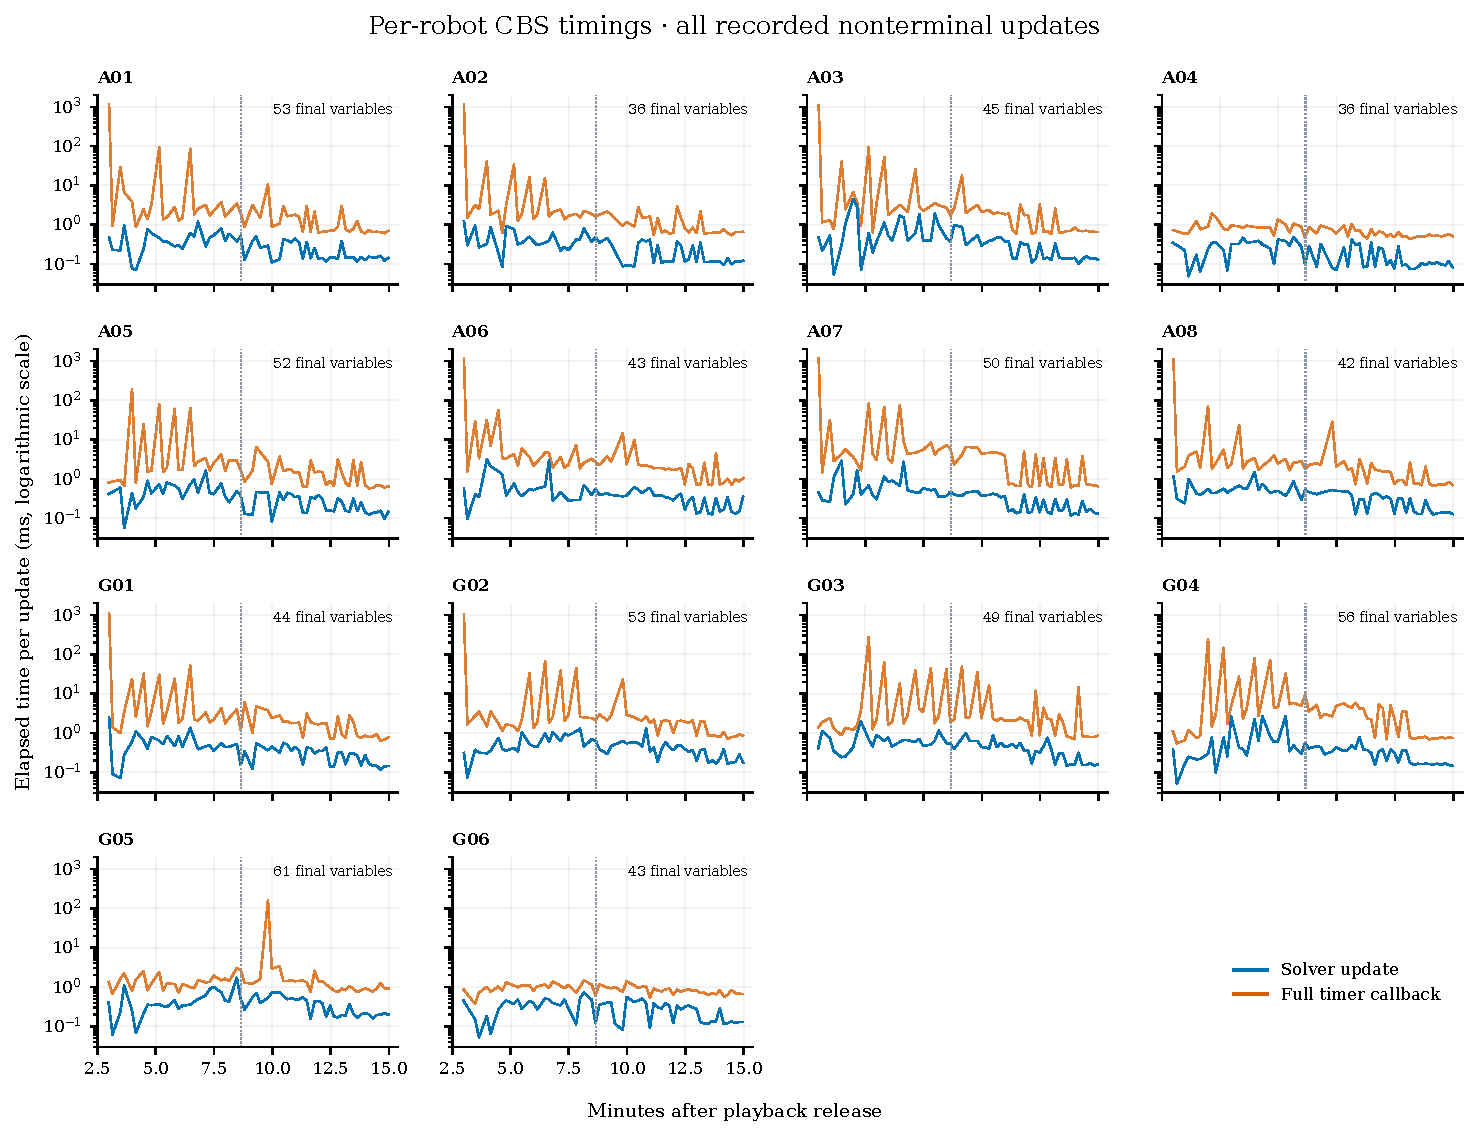
\includegraphics[width=\linewidth]{../output/pdf/cbs-per-robot-progress.pdf}
\caption{All 14 robots' nonterminal timing records. Blue is the solver update and orange the broader timer callback. Dotted lines mark the last bag's end. The logarithmic axis preserves admission spikes and low-cost updates in one view. Final variable counts include local and separator poses and anchors.}
\label{fig:per-robot}
\end{figure}
\FloatBarrier
